\chapter{Ограничения известных схем. Постановка задачи}\label{ch:ch2}

\section{Определение направлений дальнейших исследований}
Итак, в предыдущей главе был представлен анализ современных подходов к проблеме повторного обогащения регенерата.
Успехи в этой области произошли благодаря достижениям последних 60-ти лет в каскадной теории разделения многокомпонентных смесей.
Следует отметить, что успехи на этом пути подкрепляются усовершенствованием технологии ГЦ, на сегодня лидирующей в промышленном производстве обогащенного урана.

А чтобы эффективно использовать накопленный опыт для дальнейшего поиска усовершенствованных конфигураций каскадов, необходимо изучить природу ограничений имеющихся схем. Для этого в первую очередь необходима постановка расчетной задачи, в приложении к которой могут быть изучены рассматриваемые схемы.

\section{Расчетные исследования}

Начнем с очерчивания рамок расчетного исследования -- с конкретизации заданных условий к возврату регенерата для постановки численного эксперимента.
Оставляя в стороне вопросы, связанные с химической переработкой для получения восстановленной урановой изотопной смеси, предлагается рассмотрение усовершенствованных каскадов газовых центрифуг для повторного обогащения этой смеси для производства низкообогащенного урана. 

В расчетных задачах ограничимся следующими предположениями:

 \begin{enumerate}
  \item регенерированный уран получен из ОЯТ легководного энергетического реактора. В качестве примера будем рассматривать изотопный состав регенерата из реактора российского дизайна -- ВВЭР. Для моделирования многократного рецикла будут использованы исходные питающие изотопные составы регенерата второго и пятого рециклов, представленные в таблице \ref{244549}.
  \item коэффициент разделения характерен центрифуге российского дизайна и равен 1.2 для $^{235}UF_6$ к $^{238}UF_6$ \cite{smirnovObogashchenieRegenerirovannogoUrana2018}.
  \item Требуемая концентрация в конечном продукте составляет 4.95\%, что характерно для легководных реакторов.
  \item Расход регенерированного урана на единицу конечного продукта в виде низкообогащенного урана: 0,93 кг на 1 кг НОУ \cite{smirnovApplyingEnrichmentCapacities2018}.
  \item Концентрация $^{235}$U в потоке отвала по умолчанию задается равной 0.1\%.
  \item Соотношение $^{234}$U к $^{235}$U не должно превышать 0.02.
  \item Коэффициент компенсации реактивности равен 0.29 и также соответствует легководным реакторам российского дизайна \cite{smirnovApplyingEnrichmentCapacities2018}.
  \item Концентрация $^{232}$U ограничена величинами $5\cdot10^{-7}$\%, или, в некоторый случаях, $1\cdot10^{-7}$\%.
\end{enumerate}

\begin{table}[h]
  \centering
  \normalsize\begin{tabulary}{1.0\textwidth}{CCCCCCC}
  Цикл № & Массовое число & 232 & 233 & 234 & 235 & 236 \\
  2 & C, \% & 6.62e-7 & 1.19e-6 &    3.28e-2 & 1.43 & 0.9932 \\
   &  &  &  &  &  &  \\
  5 & C, \% &  1.03e-6 &   1.3e-6 &  3.91e-2 &     1.07 &     1.45 \\
   &  &  &  &  &  &  \\
  \end{tabulary}
  \caption{{Изотопные составы регенерата различных циклов{\label{244549}}%
  }}
\end{table}

\subsection{Обоснование ограничений использования ординарных схем (на основе ординарных каскадов)}

С помощью этой постановки задачи будет произведена проверка соответствия схем обогащения, основанных на ординарном каскаде, возможности решения задачи многократного рецикла.

Начнем анализ со схемы, когда регенерат второго рецикла обогащается до уровня, превышающего требуемую концентрацию $^{235}$U, а затем разбавляется природным ураном (рис. \ref{fig:diagram1}.2).

Тогда как получаемая смесь должна одновременно соответствовать требуемой величине обогащения по $^{235}$U, отвечать ограничению по $^{232}$U и удовлетворять условию компенсации $^{236}$U, то есть должны выполняться ограничения на 3 величины, связанные с этими концентрациями, управляющих параметров в такой задаче только два: выходная концентрация $^{235}$U и соотношение смешиваемых потоков. Возможность получить решение задачи при таких условиях будет проанализирована далее.  При этом важно отметить, что хоть выходная концентрация $^{235}$U и является управляющим параметром, ее изменение неминуемо влечет за собой изменение и концентраций $^{236}$U и $^{232}$U, тем самым внося дополнительную неопределенность в решение задачи.  

% \usepackage{subcaption}
\begin{figure}[ht]
  \begin{minipage}{.5\textwidth}
    \centering
    % include first image
    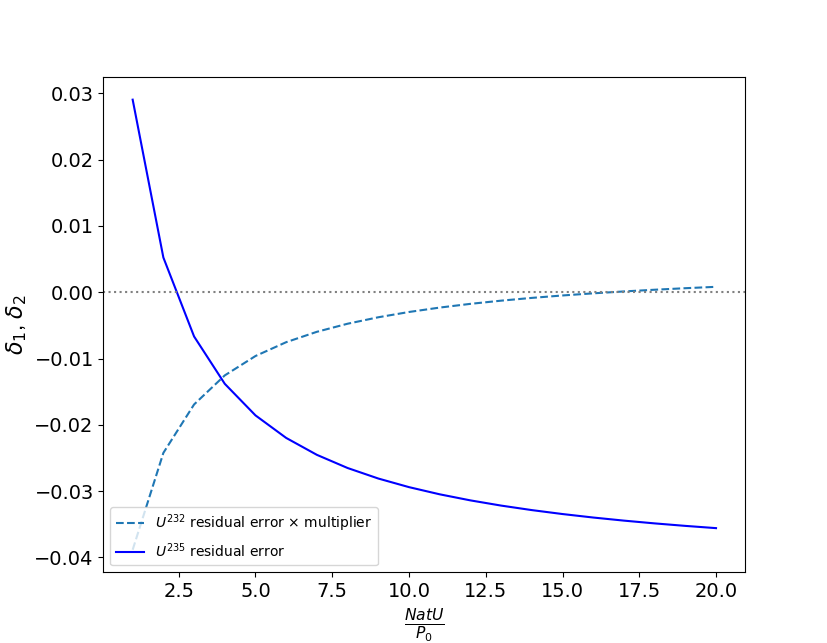
\includegraphics[width=.8\linewidth]{images/plots/15}  
    \caption{Концентрация $^{235}$U в предварительно обогащенном регенерата равна 15\%}
  \end{minipage}
  \begin{minipage}{.5\textwidth}
    \centering
    % include second image
    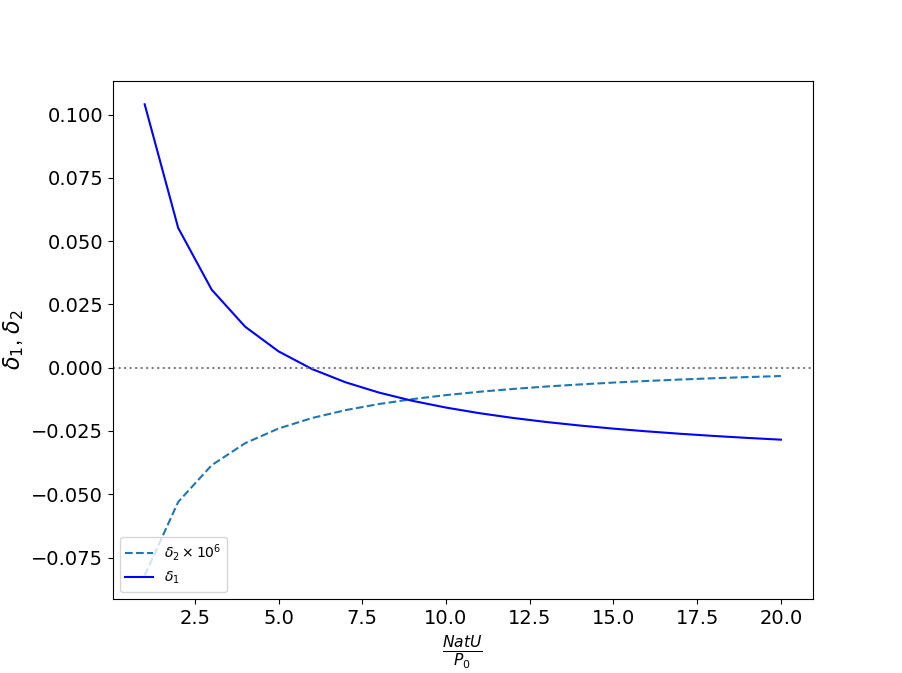
\includegraphics[width=.8\linewidth]{images/plots/30}  
    \caption{Концентрация $^{235}$U в предварительно обогащенном регенерата равна 30\%}
  \end{minipage}
  \begin{minipage}{.5\textwidth}
    \centering
    % include second image
    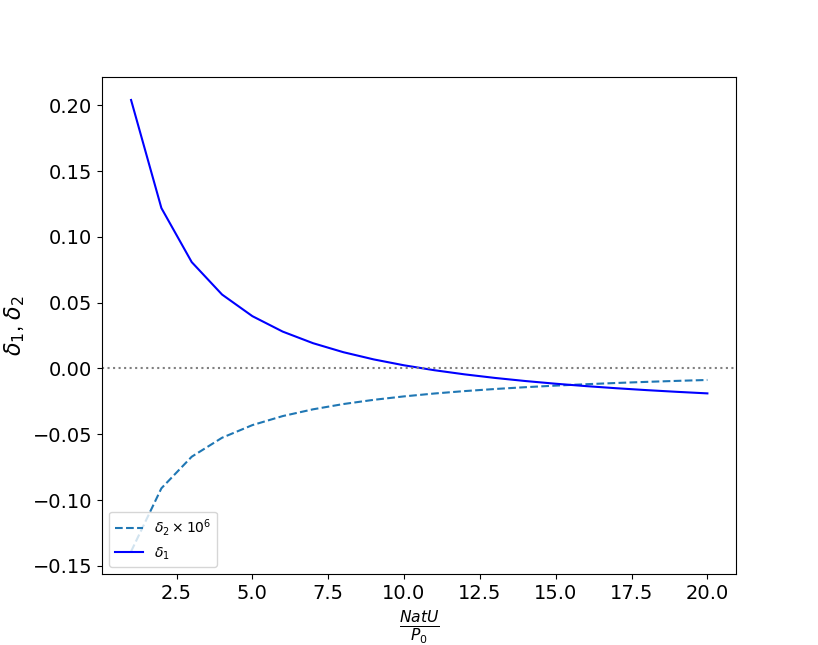
\includegraphics[width=.8\linewidth]{images/plots/50}  
    \caption{Концентрация $^{235}$U в предварительно обогащенном регенерата равна 50\%}
  \end{minipage}
  \begin{minipage}{.5\textwidth}
    \centering
    % include second image
    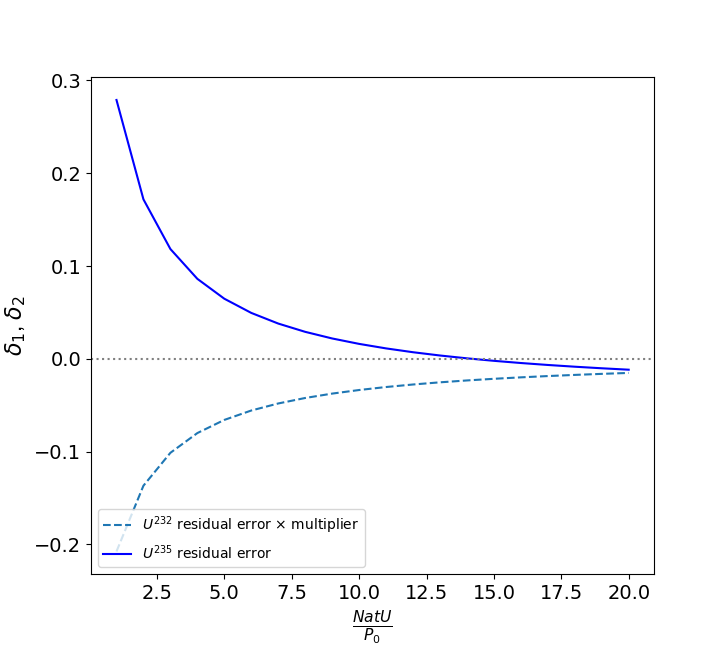
\includegraphics[width=.8\linewidth]{images/plots/65}  
    \caption{Концентрация $^{235}$U в предварительно обогащенном регенерата равна 65\%}
  \end{minipage}
  \caption{Невязки для $^{235}$U и $^{232}$U}
  \label{fig:deltas_ordinar}
 \end{figure}

Кривые рис. \ref{fig:deltas_ordinar} отражают зависимости величин

$\delta_1=\left[C_{235}^P-\left(C_n^P+RCC\times C_{236}^P\right)\right]$ и $\delta_2=\left[C_{232}^P-5\times10^{-7}\right]\times10^5$ от пропорции природного урана-разбавителя к предварительно обогащенному регенерату. Различные графики рис. \ref{fig:deltas_ordinar} построены для различных значений концентрации $^{235}$U в предварительно обогащенном регенерате. По своему физическому смыслу величина $\delta_1$ представляет собой абсолютное отклонение концентрации изотопа $^{235}$U (выраженное в долях) в окончательном продукте (после смешивания) от требуемой величины, с учетом компенсации $^{236}$U, а величина $\delta_2$ представляет собой разность фактической концентрации $^{232}$U в окончательном продукте и требуемой величины в соответствии с принятым ограничением. А чтобы сопоставить указанные величины на одном рисунке, $\delta_2$ была взята с поправкой (умножена на специально подобранный числовой коэффициент). То есть, величины $\delta_1$ и $\delta_2$ соответствуют невязкам в решении системы нелинейных уравнений, которые, в случае успешного нахождения решения системы будут равняться нулю (величине, не превышающей максимально допустимую погрешность вычислений, которая в численном методе решения задается с помощью специальной системной переменной).

Итак, для успешного решения СНАУ, обе функции должны равняться нулю для одного и того же значения аргумента, чего не удается достичь на приведенных рисунках.
Таким образом, полученные результаты показывают невозможность подбора такой конфигурации каскада (рис. \ref{fig:diagram1}.2), когда будут одновременно выполнены условия на $^{235}$U и $^{232}$U, для решения задачи в выбранной постановке. Иными словами, невозможно наладить процесс обогащения регенерата для возврата его в ядерный топливный цикл в условиях многократного рецикла на базе схемы, основанной на идее разбавления предварительно обогащенного регенерата изотопной смесью природного урана. А то, что возможность решения задачи с помощью рассматриваемой схемы зависит от состава регенерата урана, является неудовлетворительным исходом. 

Для расширения возможности решения поставленной задачи с помощью схемы на основе трехпоточного ординарного каскада, когда предварительно обогащается регенерат, необходимо заменить разбавитель--природный уран на предварительно обогащенный низкообогащенный уран, не содержащий минорных изотопов, например, изготовленный из природного урана. В таком случае будет возможно найти решение, когда будут одновременно выполнены условия на $^{235}$U и $^{232}$U (добиться равенства нулю обеих невязок). Чтобы исследовать область параметров, в которой может работать схема и где она наиболее эффективна, далее будут исследованы диапазоны двух основных параметров схемы: $^{235}$U в $P_0$ и $W_0$. Это поможет проиллюстрировать как меняются доли природного урана и регенерата в конечном продукте и как ведет себя работа разделения.

\begin{figure}[ht]
  \centerfloat{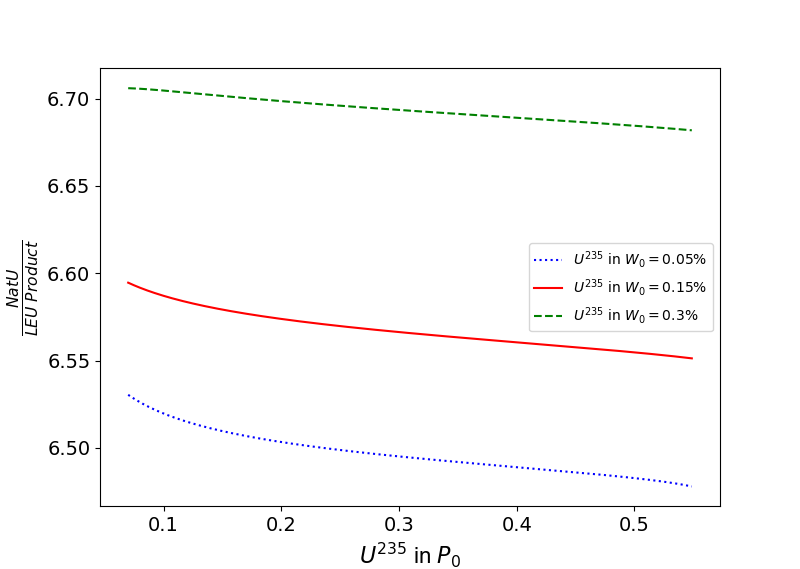
\includegraphics[scale=0.7]{images/plots/sc2_2}}
  \caption{Расход природного урана на единицу НОУ-продукта  для различных концентраций $^{235}$U в потоках продукта и отвала каскада, обогащающего регенерат}\label{fig:sc2_2}
\end{figure}

Рис. \ref{fig:sc2_2} иллюстрирует неизбежность высокого уровня расхода природного урана для производства необходимого НОУ-продукта  -- значений, близких для расхода природного урана, когда он задействуется без добавки из регенерата для производства свежего НОУ топлива. Так, для аналогичного по исходным требованиям НОУ, производимого исключительно из природного урана, эти же соотношения для природного урана, отнесенного к конечному НОУ-продукту, будут составлять $\approx$7,41 и $\approx$8,55 для $W_0$ = 0,05\% и 0,15\% соответственно. Нижний правый угол рисунка \ref{fig:sc2_2}, где $^{235}$U из регенерата обогащается до значений, превышающих пороговое значение для НОУ в 20\% \cite{brownOriginsSignificanceLimit2016}, и где регенерат обедняется в отвальной части до более низких значений (0.05\%), соответствует наилучшей конфигурации с точки зрения экономии природного урана. Более высокий уровень извлечения $^{235}$U из регенерата с более низкой концентрацией $^{235}$U в $W_0$ помогает экономить природный уран, позволяя использовать НОУ-разбавитель с более низким уровнем $^{235}$U, что проиллюстрировано на рис.\ref{fig:sc2_LEU_D} , а более высокий уровень обеднения исходной смеси ($W_0$ = 0,05\%), позволяет экономить работу разделения, что показано на рис.\ref{Figure_13} за счет более эффективного извлечения $^{235}$U из регенерата -- смеси, в которой исходно больше доля этого целевого изотопа.

\begin{figure}[ht]
  \centerfloat{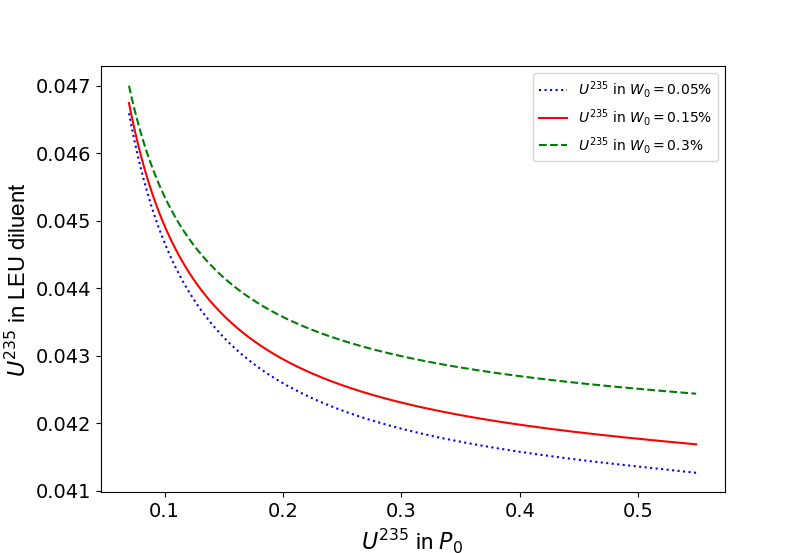
\includegraphics[scale=0.7]{images/plots/sc2_LEU_D}}
  \caption{Концентрация $^{235}$U в разбавителе, необходимая для получения свежего НОУ для различных концентраций $^{235}$U в потоках продукта и отвала каскада, обогащающего регенерат}\label{fig:sc2_LEU_D}
\end{figure}

\begin{figure}[ht]
  \centerfloat{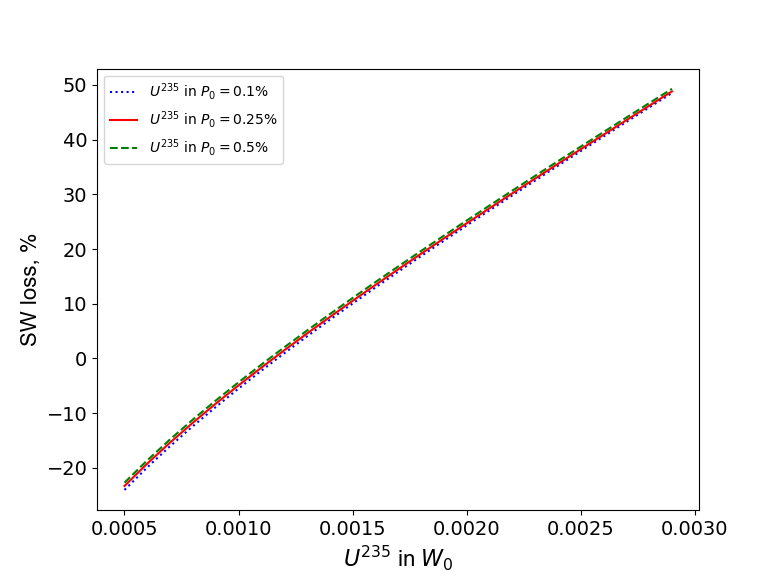
\includegraphics[scale=0.7]{images/plots/Figure_13}}
  \caption{Потери работы разделения по сравнению с ординарным каскадом для обогащения природного урана для различных концентраций $^{235}$U в потоках продукта и отвала каскада, обогащающего регенерат}\label{Figure_13}
\end{figure}

Но, как показывает рис.\ref{Figure_10}, нет возможности выполнить условия возврата заданной доли регенерата на единицу продукта. И доля используемого регенерата на единицу продукта меняется лишь незначительно с ростом содержания $^{235}$U в $P_0$. То есть, удлинение  обогащающей части каскада не приводит к существенному росту вовлечения регенерата.

\begin{figure}[ht]
  \centerfloat{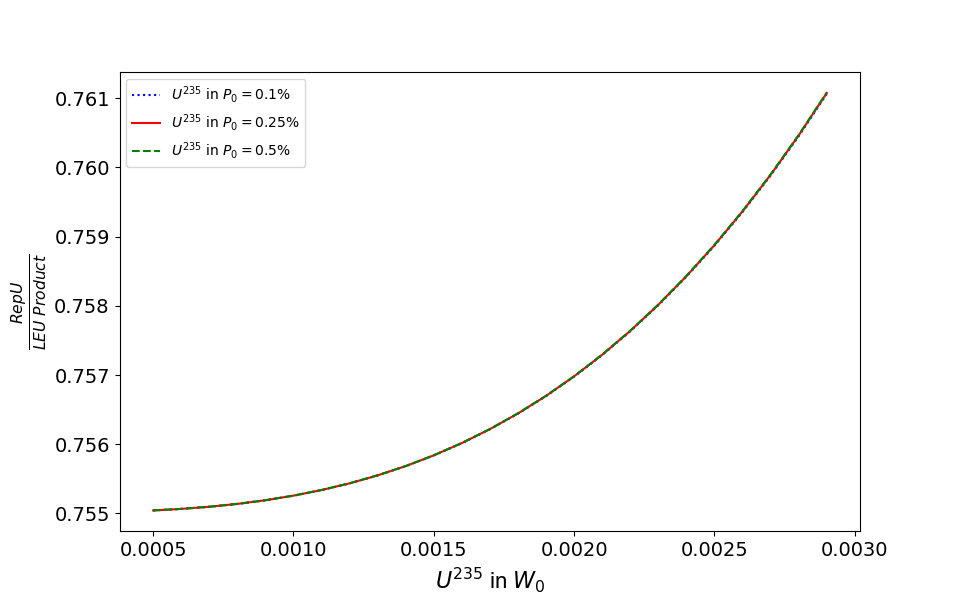
\includegraphics[scale=0.7]{images/plots/Figure_10}}
  \caption{Расход регенерата на единицу конечного НОУ-продукта для различных концентраций $^{235}$U в потоках продукта и отвала каскада, обогащающего регенерат}\label{Figure_10}
\end{figure}

Слияние кривых на рис.\ref{Figure_13} и \ref{Figure_10}, соответствующих различным концентрациям $^{235}$U в обогащенном регенерате, объясняется эквивалентностью масс $^{235}$U в каждом из этих потоков, что отражает эквивалентность вклада от обогащенного регенерата в формирование конечного продукта.

Проиллюстрировать затраты на работу разделения от составных  частей каскадной схемы, можно с помощью рис.\ref{myplot}, который показывает, что доля центрифуг для приготовления разбавителя из природного урана выше, чем доля центрифуг, задействованных для предварительного обогащения регенерата, и эта пропорция уменьшается с понижением содержания $^{235}$U в $W_0$.

\begin{figure}[ht]
  \centerfloat{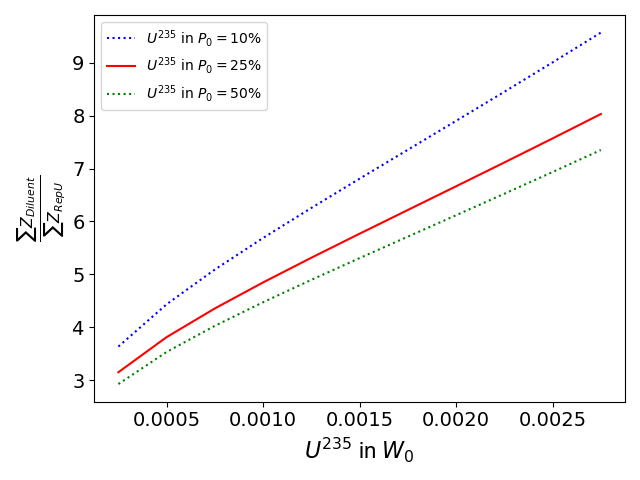
\includegraphics[scale=0.7]{images/plots/myplot}}
  \caption{Отношение количества центрифуг в каскаде, производящем разбавитель из природного урана, к количеству центрифуг, задействованных для предварительного обогащения регенерата, для различных концентраций $^{235}$U в потоках продукта и отвала каскада, обогащающего регенерат}\label{myplot}
\end{figure}


Таким образом, анализ рис.\ref{fig:sc2_2}-\ref{Figure_10} показывает непригодность схемы рис. \ref{fig:diagram1}.2 с разбавлением предварительно обогащенного урана смесью, не содержащей минорных изотопов, для решения поставленной задачи обогащения в условиях многократного рецикла, так как с помощью такой схемы невозможно вовлечь заданное количество регенерата в производство единицы товарного НОУ (0.93). При этом, анализ графиков демонстрирует, что уменьшение концентрации $^{235}$U в $W_0$ позволяет достичь наилучшей реализации схемы, изображенной на рис. \ref{fig:diagram1}.2: достичь экономии природного урана на единицу продукта (рис. \ref{fig:sc2_2}), обойтись меньшей концентрацией $^{235}$U в НОУ-разбавителе (рис. \ref{fig:sc2_LEU_D}), а также сэкономить работу разделения (рис. \ref{Figure_13}), при том что расход регенерата на единицу продукта будет меньше на незначительную величину (рис. \ref{Figure_10}), не превышающую 1\% по сравнению с каскадом для обогащения природного урана. Анализ графиков (рис.\ref{fig:sc2_2} и \ref{fig:sc2_LEU_D}) демонстрирует возможность с увеличением уровня обогащения регенерата получить б'ольшую экономию природного урана за счет меньшей необходимой концентрации $^{235}$U в НОУ-разбавителе. Однако, следует отметить, что превышение концентрации $^{235}$U уровня НОУ (20\%) может быть недопустимо на некоторых разделительных производствах, так как такой материал попадает в категорию высокообогащенного урана (ВОУ), на производство которого наложены ограничения \cite{gusevProliferationResistanceAnalysis2019}.


Перейдем к анализу схемы рис. \ref{fig:diagram1}.3, где предварительно обогащенный природный уран смешивается с возвращаемым в топливный цикл регенерированным ураном. В такой схеме на одну независимую переменную (степень свободы) меньше, поскольку мы не можем контролировать разбавитель до его смешивания с обогащенной в каскаде смесью. Таким образом, принимая жесткие требования к четным изотопам, возможно получение единственного решения. В такой конфигурации, как и в случае применения схемы рис. \ref{fig:diagram1}.2, недостаточен расход регенерата на единицу НОУ-продукта ($\approx$0,75), а уровень обогащения природного урана в каскаде достигает $\approx$16\% для разных значений концентрации $^{235}$U в отвале этого каскада. Следовательно, такие варианты модификаций трехпоточного каскада не адекватны поставленной задаче.

Еще одним вариантом реализации простейшей модификации ординарного каскада, используемого для обогащения природного урана, является предварительное смешение природного урана с регенератом перед подачей результирующей смеси на питание каскада в заданной пропорции, определяемой из ограничения на четные изотопы в конечном НОУ-продукте. Такая схема изображена на рис. \ref{fig:diagram1}.1. Для нее, как показывает анализ решений (рис. \ref{sc3_1.second}, где решениям соответствуют пересечения кривых с серыми линиями), также невозможно достижение требуемой пропорции расхода регенерата урана на единицу финального продукта. Верхняя горизонтальная ось здесь и на следующем графике (рис. \ref{sc3_2.second}) отображает долю регенерата в питающей изотопной смеси.

\begin{figure}[ht]
  \centerfloat{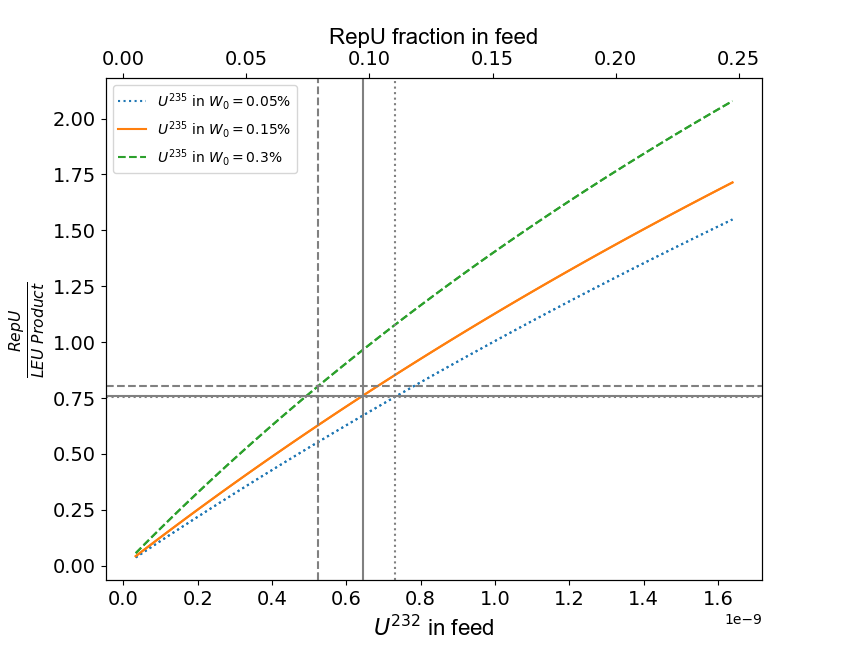
\includegraphics[scale=0.7]{images/plots/sc3_1.second}}
  \caption{Расход регенерированного урана на единицу НОУ-продукта  при различной концентрации $^{232}$U в питающем потоке каскада для различных концентраций $^{235}$U в потоке отвала}\label{sc3_1.second}
\end{figure}

Рис.\ref{sc3_2.second} показывает расход природного урана на единицу продукта для того же набора найденных решений.

\begin{figure}[ht]
  \centerfloat{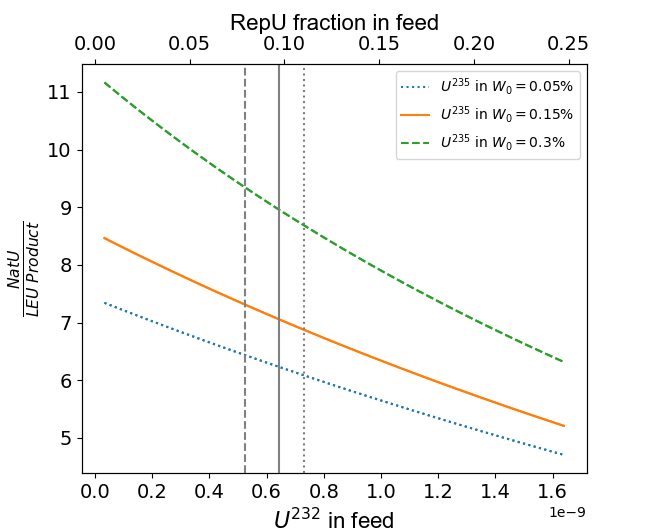
\includegraphics[scale=0.7]{images/plots/sc3_2.second}}
  \caption{Расход природного урана на единицу НОУ-продукта  при различной концентрации $^{232}$U в питающем потоке каскада для различных концентраций $^{235}$U в потоке отвала}\label{sc3_2.second}
\end{figure}


Таким образом, численные эксперименты доказали, что мы не можем использовать каскады, являющиеся простейшими модификациями ординарного трехпоточного каскада, для многократного рецикла урана. Отсюда закономерно возникает вопрос: возможно ли априорно оценить способность рассматриваемой схемы решить эту задачу? Согласно уравнениям балансов материальных потоков \ref{GrindEQ__1_21_}, из которых получен частный случай путем предельного перехода для самого легкого изотопа в ряду \ref{eq_232_balance}, достижение требуемого соотношения (1:1) облученного топлива к свежему (соответствующего 0.93 долям затрачиваемого регенерата на единицу НОУ-продукта) может быть обеспечено только тогда, когда концентрация $^{232}$U в исходном регенерате ниже, чем ограничение на присутствие $^{232}$U в конечном продукте.

\begin{equation}
\label{eq_232_balance}
  C_{232_{U}}^{P} \approx \frac{F}{P} C_{232_{U}}^{F}
\end{equation}

С помощью этого уравнения можно вычислить максимально возможную долю питающего потока, содержащего $^{232}$U, как неизвестную переменную уравнения \ref{eq_232_balance}. При этом предполагая, что весь исходный $^{232}$U окажется в конечном счете в продукте.

\begin{equation}
  \label{eq_232_balance_X}
    5 \times 10^{-7} \% \approx X \times 6.622 \times 10^{-7} \% \Rightarrow X \approx 0.755
\end{equation}

Но требуется 0,93, из чего можно сделать вывод, что полностью вернуть регенерат в топливный цикл с помощью схем простейшей модификации ординарного каскада невозможно.
Подсчитаем предельный вклад $^{235}$U от регенерата. На этот раз необходимо учитывать концентрацию $^{235}$U в потоке отвала (обедненном), так как значительное количество этого изотопа попадает в отвал каскада. Из балансных уравнений \ref{GrindEQ__1_21_} получаем:

\begin{equation}
  \label{eq_235_balance_X}
    C_{235}^{P} \approx \frac{F}{P} C_{235}^{F}-\frac{W}{P} C_{235}^{W} \approx 0.755 \times 0.01428-3 \times 0.001 \approx 0.0078
\end{equation}

Отсюда, сравнивая полученное значение с требуемой концентрацией $^{235}$U, можно вычислить предельный вклад $^{235}$U от регенерата, который будет составлять $\approx$16\% ($0.0078/0.0495\approx0.16$), что соответствует экономии природного урана. В реальной задаче, к сожалению, эта величина экономии будет еще меньше из-за необходимости компенсации по $^{236}$U.

В результате, поскольку количество $^{232}$U в исходном регенерате второго цикла исходно превышает ограничение в $5\cdot10^{-7}$\%, невозможно обеспечить возврат регенерированного урана в ЯТЦ в условиях многократного рецикла с помощью простейших модификаций ординарного каскада, где, либо регенерированный уран предварительно обогащается, либо используется как разбавитель предварительно обогащенного природного урана.
Таким образом, анализ схем на основе базового трехпоточного каскада демонстрирует потребность в модификации компоновок разделительного оборудования в контексте многократного рецикла урана.
Отсюда вытекает необходимость использовать каскады, предназначенные для отделения $^{232}$U и $^{234}$U от $^{235}$U. Такие схемы основаны на двух связанных каскадах, где в первом $^{235}$U обогащается с одновременным увеличением концентрации изотопов $^{232}$U и $^{234}$U, а во втором каскаде смесь изотопов разделяется на легкую ($^{232,233,234}$U) и тяжелую фракции ($^{235,238}$U) \cite{smirnovApplyingEnrichmentCapacities2018}.
Обзор такой схемы (рис. \ref{fig:double_ru}) представлен в первой главе.

Дальнейшая работа предполагает на основе вычислительных экспериментов и анализа закономерностей массопереноса определение схем каскадов, которые могут быть использованы для обогащения регенерированного урана в рамках многократного рецикла.

\section{Обоснование необходимости составных схем}\label{sec:ch2/sec2}
Из вышеприведенного обоснования невозможности решения задачи полного возврата регенерата в топливный цикл легководных реакторов в условиях многократного рецикла и вытекает необходимость использовать составные каскадные схемы ввиду необходимости  <<пространственного>> разделения легкой изотопной фракции с $^{232}$U, $^{234}$U от с $^{235}$U. Так двойная схема позволяет отделить минорные легкие изотопы $^{232}$U, $^{234}$U в независимом потоке отборной части каскада.
Так, например, схема (рис. \ref{fig:double_ru}) позволяет во втором каскаде разделить потоки, выделив $^{235}$U в тяжелой фракции, направив $^{232}$U и $^{234}$U в легкую.
С появлением свойств такого рода у каскадов, вместо привычной дихотомии, выделяющей схемы с приставкой <<много->> (многопоточные схемы, многокаскадные конфигурации), предлагается классифицировать каскады, используемые для обогащения регенерата, как разбавляющие или очищающие, потому что условная граница <<каскад-разбавитель>> -- <<каскад-очиститель>> гораздо лучше подчеркивает сущностные характеристики анализируемых схем, предназначенных для повторного обогащения урана. Так, схема двойного каскада является очищающей, в отличие от схем, основанных на ординарном каскаде, работающих на принципе разбавления.  

В обзоре (глава 1) диссертации было показано, что такая схема (рис. \ref{fig:double_ru}) не может обеспечить соблюдение заданной пропорции для возврата.
